\section{C5G7}
\label{sec:c5g7}

\subsection{Models and runs}

The quarter core is $51 \times 51$ pin cells of 1.26~cm (four $17 \times 17$
assemblies and a 21.42~cm water reflector), seven groups, reflective on the
two symmetry planes and vacuum outside. Three \garnet{} models were run:

\begin{itemize}
\item \textbf{Pin-resolved} (the paper's geometry): every lattice position is
  an $r = 0.54$~cm cylinder in water, on $s \times s$ cells per pin cell,
  with exact covered fractions (\code{build\_c5g7\_2d(pin\_resolved=True,
  exact\_area=True, outer\_bc="vacuum")}). With Marshak vacuum,
  $s = 4$--$48$ for SP$_N$ and $s = 4$--$24$ for SDP$_N$; Robin vacuum at
  $s = 4, 8, 16$; zero-flux outer faces at $s = 8$.
\item \textbf{Pin-resolved with sampled areas}: the builder's default
  $16 \times 16$-point sampling of the covered fractions, SP1 only.
\item \textbf{Pin-cell homogenized}: each pin cell volume-weighted, zero-flux
  outer faces, $s = 1, 2, 4, 8$. This is the model of
  \path{tests/validation/test_c5g7.py} (at $s = 1$).
\end{itemize}

Up to $s = 12$ runs were made on the CPU, from $s = 8$ on a GH200
(\code{data/runs-gh200/}). The 18 configurations run on both agree to
$1.3 \times 10^{-13}$ in $k$.

\subsection{Mesh convergence}

\begin{figure}[h]
\centering
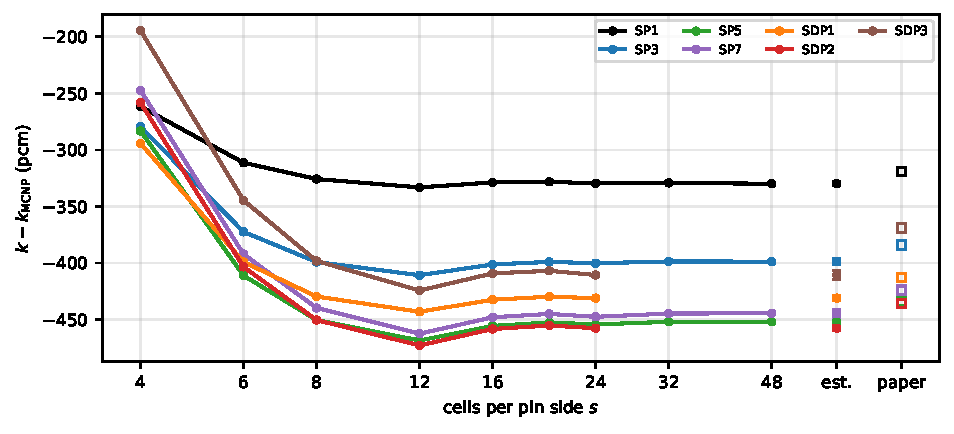
\includegraphics[width=0.85\textwidth]{c5g7_keff.pdf}
\caption{C5G7 pin-resolved, Marshak vacuum: $k - k_{\rm MCNP}$ against cells
per pin side. ``est.'' is the finest-mesh estimate with its spread over
$s \ge 16$; ``paper'' is Table~7.}
\label{fig:c5g7-k}
\end{figure}

The pin-resolved model does not converge monotonically
(Fig.~\ref{fig:c5g7-k}, Table~\ref{tab:c5g7-k}). At $s = 4$ every method is
68--216~pcm above its fine-mesh value; at $s = 12$ every method dips 3--18~pcm
below it; from $s = 16$ on the values settle. How the fuel circle cuts the
cells changes from mesh to mesh, so the blend error does not follow a power
law, and Richardson extrapolation through these points would be arbitrary.
The estimate is therefore the finest-mesh $k$ ($s = 48$ for SP$_N$, 24 for
SDP$_N$). Its uncertainty, 1.7--3.8~pcm, is the larger of two measures: the
largest difference from it among the meshes with $s \ge 16$, and its
distance to a least-squares $k_\infty + b/s^2$ fit over the same meshes.

\begin{table}[h]
\caption{C5G7 pin-resolved eigenvalues, Marshak vacuum. Paper column: Table~7
$k$ and $10^5 (k - k_{\rm MCNP})$. Differences in pcm.}
\label{tab:c5g7-k}
\tablefile{c5g7_keff}
\end{table}

\subsection{Comparison with the paper and MCNP}

For the six methods whose tables the paper and \garnet{} share (SP1--SP7,
SDP1, SDP2), \garnet's estimate is 11--22~pcm below Table~7, and the offset
grows with the number of moments: 11~pcm for diffusion, 15--20~pcm for
SP3--SP7, 18--22~pcm for SDP1--SDP2. For SDP3 it is 42~pcm. The FEMFFUSION
tables raise C5G7 SDP3 by 14~pcm at $s = 4$ (Section~\ref{sec:a6}), so with
them the offset would be about 27~pcm, in line with the other methods.

Unlike Brantley--Larsen, the two C5G7 models are not the same discrete
problem. The paper meshes each pin with second-degree finite elements
(its Fig.~5) and states neither how the circular pin boundary is represented
nor a mesh study; \garnet{} blends the cells the circle cuts, with exact
areas. The source of the 11--22~pcm offset is not identified. It is 3--5\% of
the 320--460~pcm angular error and changes none of the orderings below.

Against MCNP both codes give the same picture. Diffusion is closest
($-330$~pcm here, $-319$~pcm in the paper), and every SP$_N$ and SDP$_N$
order is further away ($-399$ to $-458$~pcm here, $-369$ to $-436$~pcm in the
paper). This is the stagnation the paper reports for C5G7: on this
lightly heterogeneous lattice, the eigenvalue is not a measure of angular
accuracy. The pin powers are.


\subsection{Modelling choices}

\begin{table}[h]
\caption{C5G7 at $s = 8$: effect of the vacuum treatment and of pin-cell
homogenization on $k$ (pcm).}
\label{tab:c5g7-eff}
\tablefile{c5g7_effects}
\end{table}

Table~\ref{tab:c5g7-eff}. The vacuum faces sit behind a full assembly width
of water, so the boundary treatment hardly matters here: Robin is 0.2--0.3~pcm
below Marshak, and the builder's default zero-flux faces are 0.2--1.4~pcm
below. The pin-area computation matters much more. With the default sampled
fractions, SP1 is 226~pcm higher at $s = 4$ and 22~pcm lower at $s = 8$ than
with exact fractions, the result of a fuel-area error of $-0.66$\% and
$+0.06$\% (finding~4 explains why sampling errs this way). Pin-cell homogenization raises $k$ by 379~pcm (SP1) to 662~pcm
(SDP2) against the pin-resolved model at the same mesh.

\subsection{Pin powers}

\begin{table}[h]
\caption{C5G7 pin powers against the NEA MCNP reference, Marshak vacuum,
finest mesh. Errors in \%; the paper's Table~7 AVG and RMSE in brackets.
AVG, RMSE as the paper's tables use it ($\sqrt{\sum e_i^2}/N$), RMS, MRE and
the largest pin error, the largest pin power (MCNP 2.498), and the assembly
power errors.}
\label{tab:c5g7-pins}
\tablefile{c5g7_pins}
\end{table}

\begin{figure}[h]
\centering
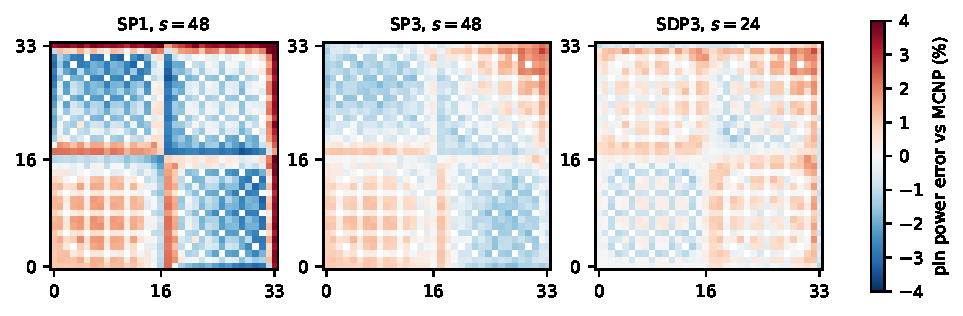
\includegraphics[width=0.85\textwidth]{c5g7_pin_errors.pdf}
\caption{Pin power error against MCNP in the four fuel assemblies (inner
UO$_2$ at the bottom left, MOX on the off-diagonal, outer UO$_2$ at the top
right).}
\label{fig:c5g7-pins}
\end{figure}

Table~\ref{tab:c5g7-pins} and Fig.~\ref{fig:c5g7-pins}. Unlike $k$, the pin
powers improve with angular order: AVG falls from 1.43\% for diffusion to
0.74\% for SP3, 0.66\% for SDP1 and 0.53--0.57\% for SP5, SP7, SDP2 and
SDP3. These are the paper's Table~7 values within 0.04 percentage points
for SP1 to SP7, SDP1 and SDP2 (SP1 1.43 against 1.43, SP3 0.74
against 0.75), and the paper's RMSE measure agrees as well. The agreement
shows that the paper scored its pin powers against the NEA MCNP reference
used here, and that the two codes' solutions match pin by pin, not only in
$k$.

For the higher orders AVG converges with mesh more slowly than $k$ and from
below: SP7 rises from 0.47\% at $s = 8$ to 0.54\% at $s = 48$, SDP3 from
0.49\% at $s = 8$ to 0.56\% at $s = 24$, still climbing. The remaining gap
to the paper for SP7, SDP2 and SDP3 (0.03--0.08 points, largest for SDP3 at
its coarser finest mesh) is consistent with that. Pin-power results from
$s \le 12$ therefore understate the converged error.

The largest pin error is 2.6--2.9\% for every transport method and 5.8\% for
diffusion. In every case it is a corner pin of the outer UO$_2$ assembly next
to the reflector, where the power is lowest (0.23--0.29) and the MCNP
reference itself is least precise. The largest pin power is within 1\% of
MCNP's 2.498, and every assembly power within 0.65\%.


\subsection{Flux along the assembly diagonals}

\begin{figure}[h]
\centering
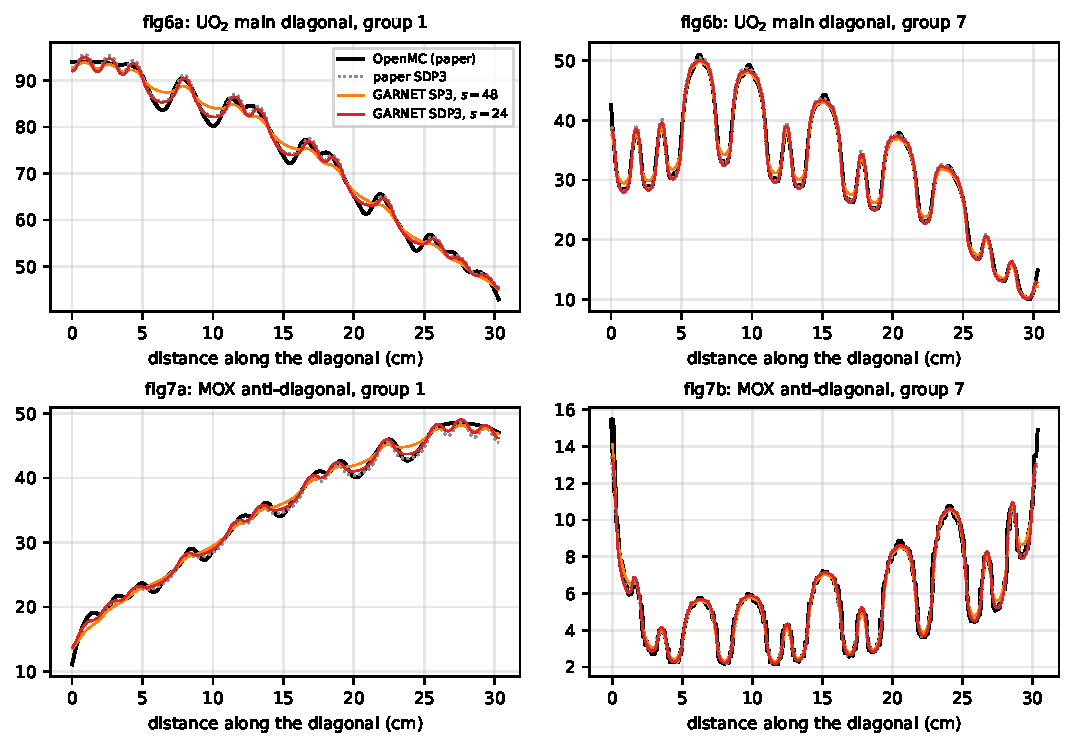
\includegraphics[width=\textwidth]{c5g7_flux_lines.pdf}
\caption{Groups 1 and 7 along the inner UO$_2$ main diagonal (paper Fig.~6)
and the MOX anti-diagonal (Fig.~7): OpenMC and the paper's SDP3, both read
from the paper, and \garnet{} SP3 and SDP3 scaled to OpenMC by least squares.}
\label{fig:c5g7-lines}
\end{figure}

\begin{table}[h]
\caption{Flux along the diagonals against OpenMC, after a least-squares scale
(\% of the OpenMC peak).}
\label{tab:c5g7-lines}
\tablefile{c5g7_flux}
\end{table}

Fig.~\ref{fig:c5g7-lines} and Table~\ref{tab:c5g7-lines}. \garnet's SDP3
deviates from OpenMC by 1.1--1.7\% of the peak (RMS) on the four panels, the
paper's SDP3 by 1.1--2.0\%: the two agree with the Monte Carlo profile equally
well, and \garnet's SDP3 is closer in group~7 of the MOX diagonal (1.7
against 2.0\%). \garnet's SP3 is further away, 1.5--1.9\%, as in the paper's
own SP$_N$/SDP$_N$ comparison. The largest local deviations, up to 8\% of the
peak in group~7, sit on the thermal-flux peaks in the water between pins and
at the reflector-side corner of the MOX assembly. The OpenMC curve is
steepest there, so these are also the points where the extracted reference is
least precise.


\subsection{The homogenized model of the regression test}

\begin{table}[h]
\caption{C5G7 pin-cell homogenized, zero-flux outer faces. $k_\infty$ from
$s = 4, 8$ at second order. Differences in pcm.}
\label{tab:c5g7-hom}
\tablefile{c5g7_homogenized}
\end{table}

The regression test's model, pin-cell homogenized at $s = 1$, lands 8--165~pcm
below MCNP (Table~\ref{tab:c5g7-hom}). The agreement is a cancellation of two
large errors. Homogenizing each pin cell raises $k$ by 380--660~pcm against
the pin-resolved model (Table~\ref{tab:c5g7-eff}), so the homogenized mesh
limit is 57--223~pcm \emph{above} MCNP and 376--650~pcm above the paper; the
$s = 1$ mesh then lowers $k$ by 222--231~pcm. The test's eigenvalue envelopes
(2\% for diffusion, 0.5\% for the family) are therefore not accuracy
statements. What those tests guard is the internal ordering of the hierarchy
and the clustering of the six transport methods, which is where the paper's
SDP2/SDP3 table errors showed.


\subsection{Solver behaviour and cost}

\begin{table}[h]
\caption{C5G7 cost, Marshak vacuum. CPU: best of three at $s = 4$, one
thread. GH200: single runs, which include CuPy kernel compilation on first
use; outer and inner counts at $s = 24$.}
\label{tab:c5g7-cost}
\tablefile{c5g7_cost}
\end{table}

Table~\ref{tab:c5g7-cost}. On one CPU thread at $s = 4$ (41\,616 cells,
seven groups) the SP$_N$ solves take 6--40~s and the SDP$_N$ solves
49--124~s. With Marshak vacuum every SDP$_N$ block is non-symmetric and runs
GMRES. At $s = 4$ its outer iteration count is still close to SP$_N$'s (64--106
against 59--68), but from $s = 8$ on it roughly doubles (121--161 against
57--73), and at $s = 24$ the inner applies are 2.9--3.6 times those of
SP3--SP7. On the
GH200 at $s = 24$ (1.5 million cells) SP$_N$ takes 30--271~s and SDP$_N$
1580--1969~s. At $s = 32$ none of the SDP$_N$ solves converged: in the first
outer iteration GMRES with Jacobi preconditioning stopped at 5000 iterations,
1.3--4.8 times above its tolerance (finding~5 in
Section~\ref{sec:findings}). The SP$_N$ solves ran to $s = 48$ (6.0 million
cells) in 2--14 minutes each.

The pin-resolved study is a GPU calculation: on the shared CPU node, with up
to 16 runs at once, the SP$_N$ solves at $s = 12$ took 14--77 minutes each and
an SDP3 solve at $s = 12$ was projected at over 20 hours.

